
\documentclass[openany]{book}
\usepackage{graphicx} % images
\usepackage{wrapfig}
\usepackage{listings} % nice code layout
\usepackage[usenames]{color} % color
\definecolor{listinggray}{gray}{0.9}
\definecolor{graphgray}{gray}{0.7}
\definecolor{ans}{rgb}{1,0,0}
\definecolor{blue}{rgb}{0,0,1}
% \Verilog{title}{label}{file}
\newcommand{\Verilog}[3]{
  \lstset{language=Verilog}
  \lstset{backgroundcolor=\color{listinggray},rulecolor=\color{blue}}
  \lstset{linewidth=\textwidth}
  \lstset{commentstyle=\textit, stringstyle=\upshape,showspaces=false}
  \lstset{frame=tb, tabsize=2}
  \lstinputlisting[caption={#1},label={#2}]{#3}
}
\renewcommand{\chaptername}{Lab}
\newcommand{\WrapBarrier}{$\quad$\vspace*{-.225in}}


\title{ELC 3338 Project Book}
\author{Steve Potter}


\begin{document}

\maketitle
\tableofcontents


\chapter{Program Counter Register}

During the course of this semester, we will build a 64-bit computer so that we can understand how it works.  To do this, we will make a synthesizable machine in Verilog, a common hardware description language (HDL).  

A computer runs a program by executing individual instructions in sequential order.  The instructions are stored in memory and are accessed by their memory address.  During each clock cycle, an instruction is fetched from memory and executed on the processor.  The memory address of the next instruction to fetch is stored in a register called the Program Counter (PC).  During Lab 1, we will build and test the Program Counter register.  In Lab 2, we build an incrementer (to count to the next instruction) and a mux (to select between the incremented count or a new starting value).   

\section{Program Counter Register}

In order to make the Program Counter, we are going to make a Verilog module that explains how to build a register (a D flip-flop).  Let me unpack the previous sentence:
\begin{enumerate}
	\item Verilog is a Hardware Description Language (HDL).
	\item We write Verilog code to tell Vivado how we want our register module to behave.
	\item Vivado reads our Verilog code and synthesizes a realizable digital hardware design that meets the behavior that we specified.  Thank you Vivado!
	\item Vivado also simulates the behavior of the hardware, allowing you to test your design without building/programming hardware.
\end{enumerate}   
Consider the Verilog code in Listing~\ref{code:register}.  It is made up of three sections: a header (which has the include command), a port list or interface (which specifies the signals coming in or going out of our module), and a body or implementation (which describes how to build it).

\Verilog{Verilog code to make a register.}{code:register}{../code/1_fetch/register.v}

The first part is the header.  We will use this same header each time.  It tells the Verilog compiler to get all the data from a file called definitions.vh.  The extension vh is a Verilog header.  We use this to specify common pieces of data we will use across our design, so that all the components we build will be consistent.  By putting them in one file, we make it easier to maintain, and prevent mistakes that can happen easily by having multiple copies of these basic pieces of data.  For our first component the piece of data we will be using is WORD (set to 64), which is the size of the memory addresses our computer will use (how many bits).  Note that if we build things based around WORD, rather than the number 64, we can just change the value of WORD in the file and get a computer with a different size with a couple key strokes.

The second part is the port list or interface.  In this area we specify what signals are coming in (input), going out (output), or could go either direction (inout).  Ports can be defined as either "wire" or "reg".  This can be confusing to some students.  Think of it this way: 
\begin{enumerate}
	\item Wire
	\begin{enumerate}
		\item A wire is just a conductor that connects one component or module to another.
		\item The value on a wire can only be changed by using combinational logic.
		\item It has no memory, meaning that the value on the wire is driven by the results of combinational logic at that particular moment.
		\item Module inputs are always wires
		\item Module outputs can be wires or regs.
	\end{enumerate}
	\item Reg
	\begin{enumerate}
		\item A reg more closely resembles a variable in software programming languages.
		\item A value of a reg can only be set by using sequential logic.
		\item A reg has memory, meaning that the value of the reg will remain the same until a sequential logic element updates it.
		\item You can directly set a reg to a value using a procedural assignment.
		\item Regs can be used internally in a module (neither input nor output), or they can be used as module outputs.  They cannot be used as module inputs. 
	\end{enumerate}
\end{enumerate}

\begin{figure}
	\caption{Module Diagram.}\label{fig:modulediagram}
	\begin{center}
		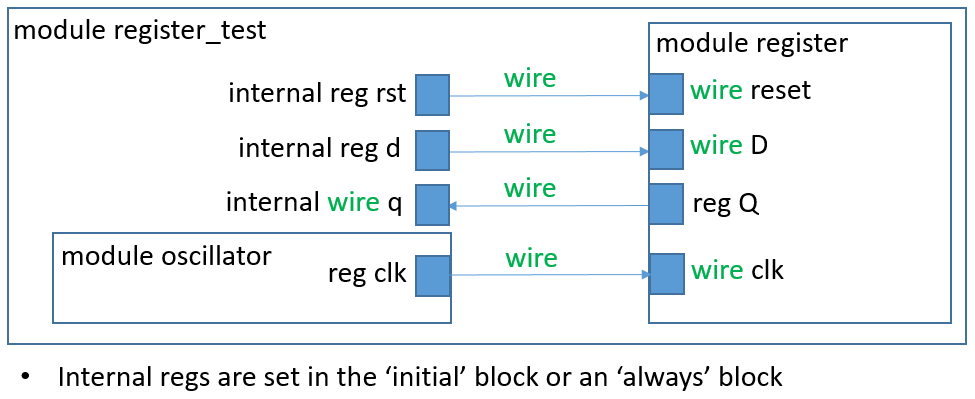
\includegraphics[width=4.75in]{../images/register_test_module_diagram.png}
	\end{center}
\end{figure}

If you don't specify anything for the port type, you will get a wire - it is the default.  In our case we have four signals: three inputs, and one output that is a register.  The first two inputs are single-bit wires.  One is the clock, which specifies the timing, and the other is reset, which clears the contents of the register (makes them zero).  The final input is the value we want to store in memory, and I have called it D, following the convention of digital logic.  D has multiple bits that are numbered from WORD-1 down to 0.  Thus the leftmost bit is 63 in this case, and the rightmost bit is 0\footnote{If you want to be technical this is called little endian, since the little end (the least significant or unit bit) is going into the first memory location (bit 0).  If you reversed the order by putting the 0 first and the WORD-1 last it would be big endian, since the big end (most significant bit) would go in the lowest addressed bit.}.  The output Q (also the digital logic conventional name) is a register (it will hold its value) and should also be of size WORD and follow the same order as the input D.

To help clarify this, please examine Figure~\ref{fig:modulediagram}, which shows the interconnection of the modules in this lab.

The final section is the body or implementation.  It is composed of a single thread of code, that will keep running (hence always).  It will run one time every time there is a positive edge (0 to 1 transition) for either the clock or reset.  Reset has higher priority, so if reset is asserted the register is cleared (Q is set to zero), otherwise the value of D is stored it Q.  That is it.  A nice, simple module.  Please note that the provided register module is fully operational.  You do not need to modify it.

\section{Testbench}

We now want to test this.  To test it, we need to tell the simulator to build a copy (instantiate) the module, and then we will need to supply the inputs and look at the outputs to verify that the module works correctly.  Consider the testbench in Listing~\ref{code:register_test}.

\Verilog{Verilog code to test a register.}{code:register_test}{../code/1_fetch/register_test.v}

Like our register it starts with our standard header, but this time there are no ports!  A testbench is providing all the signals to simulate the inputs to the unit under test (UUT) and thus does not need them.  This is how Verilog finds a top level simulation module - there are no ports.  The clock signal will be driven by a module named oscillator, which will give us a nice square wave with period CYCLE, which is another constant defined in our definitions.vh file.  The code thus makes an oscillator and a register, then runs the 'initial' section (it runs once at the start then never again).  The initial section sets the value of the inputs then waits a CYCLE.  The last couple of delays are not full cycles.  I did this for two reasons:
\begin{enumerate}
\item To show you how to make Verilog do calculations for you.
\item To remind you that the input won't necessarily be nice and perfectly timed to your register.  Unsynchronized signals happen, and is a frequent cause of problems, hence the need to test.
\end{enumerate}
This is by no means an exhaustive testbench, but run it and look at the output.  Does it do what you expect?  What else might you want to test?  Add this to your testbench and run it again to see if the register works.



\begin{figure}
\caption{Timing diagram.}\label{fig:registertiming}
\begin{center}
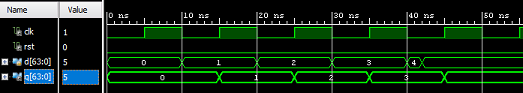
\includegraphics[width=4.75in]{../images/register_test_timing_diagram.png}
\end{center}
\end{figure}

\section{Using \LaTeX\ for Your Write-up}
This section was originally written by Dr. Schubert, so any first person references are from Dr. Schubert.

All that is left is to write it up.  I am going to have you use \LaTeX\ to do your lab reports. Note how I include files, programs, and images.  It is worth noting that \LaTeX\ will automatically make the table of contents and bibliography for you also.

Why use \LaTeX\ ?  There are lots of reasons, but here are a few that matter in this course:
\begin{enumerate}
\item It typesets programs from the actual source, no need to copy the program and have spell checkers and grammar editors mess things up.
\item It quickly and correctly handles equations.
\item It automatically handles table of contents and bibliographies.
\item It is free, and generates high quality documents (book quality) - it is open source since before open source.
\item It is used in publication of research documents.
\item It is the only large program believed to be error free in its source code, and have no missing features (development is complete!)
\end{enumerate}


\subsection{Background}

\TeX\ refers to both a language for typesetting and the program (compiler actually) that does the typesetting.  \LaTeX\ is a macro package which sits on top of \TeX\ and provides additional functionality, and has become synonymous with the language variant (dialect) of \TeX\ which it created.  Since \LaTeX\ is hugely popular and really useful, \TeX\ and \LaTeX\ have become synonymous to most people, and I will treat it so from now on.  A note on pronunciation: \TeX\ is in Greek letters - tau epsilon chi and hence is pronounced `tek' not tex (similar for \LaTeX\, which is pronounced `lay-tek' not latex).

\TeX\ is not a WYSIWYG (what you see is what you get) typesetting program like many editors you are familiar with, as it was designed to be a tagged language like the more recent html (yes, \TeX is older).  The idea is not to spend time thinking about how it should look, but rather to classify what it is and let the automated standards set the text by what the text is\footnote{For instance, note the chapter, section, and subsection commands in the tex files.  \LaTeX\ assigns a number, records it, the title, and page so it can automatically put it in the table of contents for you.}.  To provide flexibility and extension (and it was designed by one of the greatest computer scientists, Donald Knuth) it was set up as a programming language with a compiler.  Since \LaTeX\ is a programming language, we have a comment character \% that I had to escape by putting a \textbackslash before it to make it print.  Whitespace past the first space (word separation) is ignored, except for a blank line, which means start a new paragraph.  More than one blank line is ignored.  To get more space, you issue a command, such as \verb1\vspace{.25in}1, which puts a quarter inch of vertical space.  \LaTeX\ also knows pt (points), px (pixels), pc (pica), mm (millimeters), cm (centimeters), em (width of an `m'), and many more.  By default the space is not placed if it does not separate some object (i.e. at the top of a page), but you can force it by using \verb1\vspace*{.25in}1.  Starred commands are just versions of the main command.

There are many more commands than we could describe in this brief intro, including commands to let you define new commands and environments.  We will not need too many fancy commands, we only need to describe the commands to include figures, code, and equations.  If you want to learn more, then I have links to free manuals online at r2labs.org.

\subsection{Compile Process}

One thing that will help you a lot in working with \LaTeX\ is how the compile process works.  \TeX\ is a two pass compiler, but it does only one pass each time it runs.  Allow me a brief introduction to compilers, which is a great course if you can take it.

When you are compiling a file you have control statements (branches, loops, conditional execution statements like if or switch/case) that require you to know how many program lines ahead or behind something is in the assembled code, which you will not know at the start.   While you are often just putting in a flag or label to be handled by the assembler later, you in truth don't even know if they actually put the destination of the transfer of control, and thus have an error.  One easy way of handling this is to run through the process twice, collecting labels and such the first time and then doing the compile the second time through, which is what a two pass compiler does.  \TeX\ collects all the labels, notes all the chapter, section, and other structures, identifies all the bibliography references, and so on and puts them in a special auxiliary file for the next pass.  It will also create a DVI file, which has most things right, but will lack table of contents, references, bibliography, and such.  The second time through it already has the information before the file runs so it reads that first and uses it to create a fully correct output.

A logical question at this point is why not just have it run twice on its own?  Well, in the 1980's computers were small and slow, so each run of \TeX (we didn't even have \LaTeX\ at first) took an appreciable amount of time.  If you know the compile process, there are times you only have to run things once, like small spelling changes not in a title, chapter, etc.  Allowing people to do only one pass at a time was a big advantage (some \TeX\ compiles I had to do could take 10 minutes even in the 1990's).  Bibliographies are handled by an external program called BibTeX, which reads the .aux file to find the references (thus you need to run \LaTeX\ first), then pulls the data from the .bib files you specify in the calling command in your .tex file and creates a .bbl file.  The .bbl file contains all the info formatted how the bibliography should look.  \LaTeX\ reads this in the first pass and copies it over to the .aux file and resolves the links to the text references.  The next run of \LaTeX reads all this in and places both the bibliography and the cross references.  This means that to get a bibliography in you must run \LaTeX\, BibTeX, \LaTeX\, then \LaTeX\ once more.  You only need to do this if you add new reference, which in the labs will be once, provided you don't delete those intermediary files.

\subsection{Getting Started with LaTex}

Now that you have some background knowledge, we need to learn how to build a document on your computer.  There are many ways to do this, including text editors and command line tools.  I prefer using a more user-friendly editing and buidling environment.  While there are numerous options available, I choose to use TexStudio.  It is installed on all ECS computers, and it is available for free download at home.  For each lab, you will want to make a copy of LabN.tex and name it Lab1.tex, Lab2.tex, etc.  After creating Lab1.tex, I would recommend opening Lab1.tex and building it before making any changes.  Then make some changes, rebuild, and view those changes in the PDF that is generated.  Steps to build a document in TexStudio are:
\begin{enumerate}
	\item Open TexStudio on your lab computer
	\item Use the menus open Lab1.tex
	\item Click on the double green arrow icon near the top.  If you hover over it, it says "Build \& View".
	\item This should produce a PDF document on the right side of the TexStudio window
\end{enumerate}

This document should build properly as long as you don't modify it.  Once you start editing, it is possible that you will get compile errors.  These errors are listed in the bottom pane of TexStudio.  Like many compilers, they are sometimes cryptic and don't lead you directly to the problem.  The most common problem (by far) is using an underscore with using the escape character (backslash) first.  For example, look at the fetch1.tex file to see how I made this  example\_of\_how\_to\_use\_underscores.

Note that all code and image references are relative to where the .tex document is located in the file system.  It is important that you maintain the same file structure that I gave you so that these references are simple and consistent.

\section{Your Assignment}

You are to:
\begin{enumerate}
\item Finish the testbench in Listing~\ref{code:register_test} by testing several additional cases.  For instance, what happens when D is set at different points during the clock cycle, or if D is set for longer than a single clock cycle.  Also, reset is not currently being tested.  Does reset work properly?  Does the register work properly after reset has been cleared?
\item Create an Expected Results Table for your testbench.  An example Expected Results Table is at ARM-Lab/testfiles/Lab1\_Register\_ExpectedResultsTable.xlsx.  The idea behind the Expected Results Table is that you identify how you think the system should operate.  If you don't know how it should work, you will not know whether your simulation results are correct.
\item Run a simulation and generate a timing diagram.
\item Write up a lab report in \LaTeX\ following the lab format in \verb1LabN.tex1 and generate Lab1.pdf.
\item Upload Lab1.pdf file to Canvas.
\end{enumerate} 

\chapter{Program Counter Incrementer and Mux}

As mentioned in the last lab, the program counter is a register that is one word in length.  It holds the address in memory of the next instruction to be fetched and executed.  There are several ways that the program counter is updated:  
\begin{enumerate}
	\item If the program does not branch (via an if statement, while loop, etc), then the program counter should advance to the next address (add 4 bytes) each clock cycle.
	\item If the conditions of a conditional branch are met, then the program counter should be updated with the branch destination address.
	\item If an unconditional branch or jump occurs, then the program counter should be updated with the branch destination address.
	\item If an interrupt or error occurs, then the program counter should be updated with the interrupt or error handler address.
\end{enumerate}
The instructions will be fetched in sequential order the majority of the time.

\section{Incrementer}

We will build a program counter incrementer by making a simple adder.  Later in our computer we will need another adder, so we will re-use this code.  When used as the program counter, we will pass it a 4 because each instruction is 32-bits long (even though it is a 64-bit computer) and we want to increment to the next instruction in memory.  Most machines are byte addressable, because one ASCII character (a char in c/c++) is a byte.  For a machine with 32-bit instructions like we are using, that would mean that each instruction would be 4 bytes later in memory ($32/8=4$ bytes).  Therefore, we will be adding 4 to the program counter each time we want to increment the program counter.

An adder is very simple in Verilog.  There are two inputs (the two numbers to be added) and one output (the result).   All the ports are size word because they hold integers.  

In this lab you will make your own adder and a testbench for the adder.  Your adder module should be called 'adder' and should have inputs of \verb1a_in1 and \verb1b_in1.  The output should be \verb1add_out1.  HINT: this should be very easy.  Verilog is a Hardware Description Language, so use Verilog to describe what you want to do.  Don't make it complicated.  The adder code should be stored in ARM-Lab/code/0\_common/adder.v.  You will need to create this file.

\section{Input Selection via Mux}

We will also need to be able to choose between normal advancing (sequential stepping) and branching (loops, if statements, etc.).  We will use a multiplexor (mux) to do this.  A mux is a simple device that connects one of the inputs to the outputs based on how the selector bit is set.  If the selector is 0 then input 0 is connected to the output, and if the selector is 1 then input 1 is connected to the output.  One interesting addition in this block of code is the addition of a size parameter.  Parameters are passed before the normal ports and are used to configure the code to meet a requirement at the time of construction.  Note parameters are constants and cannot be changed later in the module.  The $=8$ defines the default value if nothing is specified.  In this case we are using parameters to set the number of wires that compose the inputs and output.  In our problem we will need some muxes to switch entire words (64 bits), but later we will also need to switch register addresses (5 bits).  Rather than write two muxes, we will make one and then use the parameter to change the size when they are declared.  The mux starter code is located in ARM-Lab/code/0\_common/mux.v.

\Verilog{Verilog code to make a mux.}{code:mux}{../code/0_common/mux.v}

Create a testbench for the mux.  Note that if the parameter is not set by the testbench, the mux module will set the inputs and outputs to be the default of 8.  We are going to change this to test it as a 64 bit mux.  In your testbench, instead of creating your mux module using \verb1mux UUT(...1, define the parameter as 64 by changing it to be \verb1mux#(64) UUT(...1  You can also do the dot notation as was done for the ports, but there are usually so few paramters you don't need to.  Now come up with good values to test your mux so you are confident it works.

\section{Expected Results Table}
\begin{figure}
	\caption{Expected Results Table}\label{fig:ert_adder_test}
	\begin{center}
		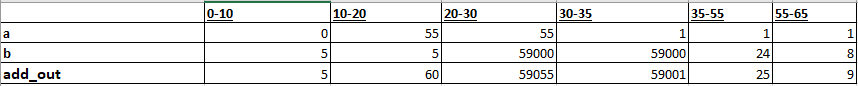
\includegraphics[width=4.75in]{../images/ert_adder_test.png}
	\end{center}
\end{figure} 
In order to verify that our modules work properly, we will create an Expected Results Table and compare our expected results with our simulation results.  The Expected Results Table is not only critical for your own verification of your module, but it is also something that I will use heavily in grading the lab reports.  In your lab reports, I need to be able to easily compare your expected results with your actual results.  Of course, I will examine your test bench code as well so that I can check that your expected results are correct as well.  The Expected Results Table should be done in Excel.  It should have simulation time values across the top and signal names along the left-hand side.  The order of the signal names in your table must match the order of the signal names in your simulation results.  Then you should fill in each block of the table with the expected value for that particular signal at that particular time.  Please use decimal numbers for all values in the expected results and the simulation results. See Figure \ref{fig:ert_adder_test} for an example Expected Results Table.

\section{Your Assignment}

You are to:
\begin{enumerate}
\item Write an adder.	
\item Write a testbench for the adder.
\item Create an Expected Results Table for the adder.
\item Update the mux starter code to operate as a mux.
\item Write a testbench for the mux.
\item Create an Expected Results Table for the mux.
\item Run a simulation and generate a timing diagram for each testbench.
\item Compare your Simulation Results with your Expected Results Table and resolve discrepancies.
\item Write up a lab report in \LaTeX\ following the lab format in \verb1LabN.tex1 and generate a pdf file.
\item Upload the pdf and all the Verilog files to Canvas.
\end{enumerate} 
\chapter{Fetch Stage}

We are ready to build our fetch unit.  To do this, we will make one more module, our instruction memory.  Then we will make a module to assemble all of our units together.


\section{Instruction Memory Module}
The instructions are stored in memory, and are accessed by using the address where they are stored.  You can think of memory like a giant hotel for our data.  Each piece of data is stored in a room (memory location), which we can find by its room number (memory address).  To get a piece of data stored in memory (like an instruction) we need to take its address, go to that location, and grab the data.  In Verilog, a bunch of memory locations that are accessed by an address is called an array.  Arrays in Verilog are declared like they are in C; the data type is specified, then the name, then the array size.  To store the instructions, we will need an array of 32-bit numbers (definitions.vh defines INSTR\_LEN as 32), which means the data type must be \verb2reg[`INSTR_LEN-1:0]2.  After the name is specified (imem in this case), we are going to use a parameter called SIZE to specify how many elements the array has: \verb2[SIZE-1:0]2.

The other interesting thing about this code is how to initialize the memory.  The default size of the memory is 1024 elements, so we do not want to initialize this memory element by element in the code.  Fortunately Verilog gives you two functions to do this automatically: \$readmemb and \$readmemh.  The last letter specifies the base (binary or hexadecimal) of the data in the file.  White space separates fields, but the underscore character is ignored and thus can be used to make the values in a number more readable.  The readmemb function will be used to read the file `IMEMFILE and store the bits in the imem array.  This is done one time on initialization.  Then, you can access that data in imem at any time after that.

`IMEMFILE is defined in definitions.vh, and I provide this file, which contains instructions.  However, you will need to update definitions.vh to point to your testfiles section rather than mine, or else it will look for mine and  not find the file.	

\Verilog{Instruction Memory}{code:instmem}{../code/1_fetch/instr_mem.v}

Starter code for the instruction memory module is given in Listing~\ref{code:instmem}.  There is only one line of code missing from this code.  Fill in the line of code inside the always block to complete the module.  Write a testbench and expected results table.  Verify that it operates correctly.  In order to confidently verify correct operation, you are required to create an Expected Results Table for your testbench and compare your simulation results with it.  Please show the instruction values in hexadecimal in the Expected Results Table and the Simulation Results.

\section{Fetch Stage}
Now we need to connect it together.  The components of our instruction fetch (sometimes called ifetch or just fetch) stage are shown in Figure~\ref{fig:fetch}.

\begin{wrapfigure}{L}{2in}
\caption{Instruction Fetch Stage.}\label{fig:fetch}
\begin{center}
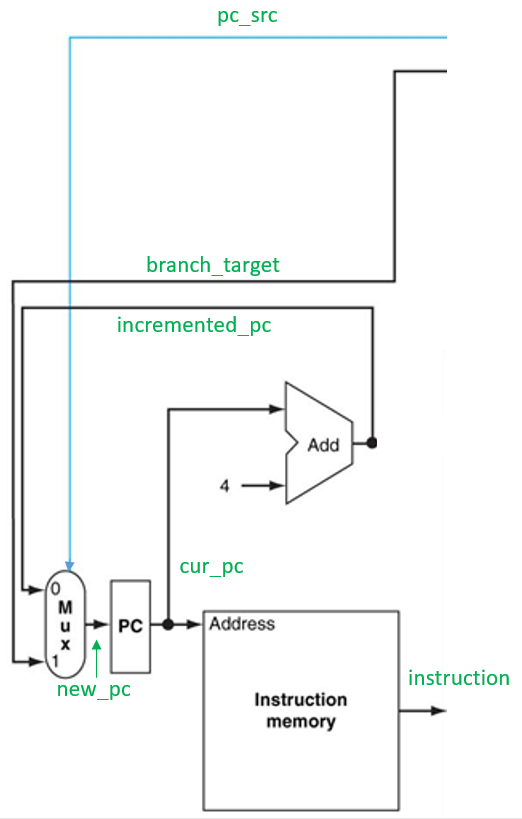
\includegraphics[width=2in]{../images/pipeline_fetch.png}
\end{center}
\end{wrapfigure}

Any wire (or reg) that comes into or goes out of the figure are input or output ports of the iFetch module.  In Figure~\ref{fig:fetch}, the blue wire is a control signal and comes ultimately from the control unit, which you will build in the decode stage.   Wires (or regs) that are completely contained in the figure are local to the iFetch module and are thus defined internally in the module.  The one exception to this is the current program counter (cur\_pc).  While there is no reason (at this point) that it must be output from the iFetch module, I strongly recommend making it an output so that it shows up on your simulation results, helping you to keep track of which instruction is currently executing.  Also, it will be required when we start pipelining our datapath in Lab 12.

While the input and output signals are easily identified by the diagram, you must also determine the size of each signal and whether it is a wire or reg.  When you look at the figure I cut from a figure in the book, note that I labeled every wire on the diagram in green.  For the sake of consistency and debugging, it is required that you use these names.  

IMPORTANT NOTE: Throughout your entire project, your signal names should follow the convention of the Freescale Semiconductor Verilog guide, which states that signal names should be all lower case, with words separated by an underscore.   

Once you have figured out all your connecting signals (wires and regs), you should identify the components you are going to use.  We have already created the modules, so now we just need to tell Verilog to instantiate them in the iFetch module and connect them together.  Create the iFetch module in a new file called iFetch.v in the code/1\_fetch directory.  

\section{Fetch Testbench}
Once you have made your connections, you should test the operation of the iFetch module by creating iFetch\_test.v.  You know you checked your individual modules, but there could be errors, or unexpected behavior when you put them together.  Sometimes weird timings between modules causes signals to be missed and such.  

Your testbench should create an instance of the iFetch module, set the inputs into the iFetch module, and verify that the correct outputs are produced. You should test both sequential operation (PC incrementing by 4) and branching.  When you test branching, keep in mind that my provided instruction file (instrData.data) only contains 14 instructions, so don't branch beyond the end of the file.

As we progress through this lab, you will learn how critical timing is.  Please look at the cur\_pc value and the instruction value and verify that the instruction that was fetched is the correct instruction, according to instrData.data and the current program counter.  Note that no instruction should be fetched in the first 5ns, as this is a half clock cycle and does not have a rising edge.  I have included a file called delay.v in code/0\_common.  It includes a module that inputs a clock signal and outputs a clock signal that is delay by some number of ns.  This will be useful when resolving timing issues.  Make sure to switch back and forth between sequential and branching to make sure that this works properly.

In order to confidently verify correct operation, you are required to create an Expected Results Table for your testbench and compare your simulation results with it.


\section{Your Assignment}
You are to:
\begin{enumerate}
\item Finish the instruction memory module.
\item Write a testbench for the instruction memory module.
\item Create an Expected Results Table for this testbench.
\item Verify the results of this testbench by comparing the Expected Results Table with the Simulation Results.
\item Finish the fetch stage.
\item Write a testbench for the fetch stage.
\item Create an Expected Results Table for this testbench.
\item Verify the results of this testbench by comparing the Expected Results Table with the Simulation Results.
\item Write up a lab report in \LaTeX\ following the lab format in \verb1LabN.tex1 and generate a pdf file.
\item Upload the pdf and all the Verilog files to Canvas.
\end{enumerate} 
\chapter{Beginning to Decode}

\section{Instruction Decode}

The next stage in the datapath is the iDecode stage.  The iDecode stage evaluates the binary instructions (an output of the iFetch stage) and determines what needs to be done.  There are many aspects to the iDecode stage, and some get fairly complex.  But today we will begin the process of decoding an instruction by decomposing the instructions into the key parts of R-Type and D-Type instructions:
\begin{enumerate}
	\item opcode
	\item address (used only in D-Type instructions)
	\item rm\_num (used only in R-Type instructions)
	\item rn\_num
	\item rd\_num (though the book uses Rt for D-type instructions, we will use Rd for the last operand of D-type instructions)
\end{enumerate}   

To do this, you will create a new module called instr\_parse.  This module will simply read inputs and assign appropriate output values.  These outputs should be assigned using continuous assignments.  The input is a 32-bit instruction.  Outputs are listed for you above.  Although R-type and D-type instructions have different operands, you can treat them the same for now.  For instance, you can still assign an Address field on an R-type instruction, and you can still assign an Rm field on a D-type instruction.  When we create the Control Module in a future lab, the control signals will drive what fields of the instruction are used and what fields are ignored.  Notice how, because of the commonality of instruction format, Opcode, Rn, and Rd are all universal across these instruction types.  Please remember to use the style specified in the previous lab, where all items are lower case with underscores separating them.  For instance, for Rd, you should use the signal name rd\_num.  Appending num on the end of the name indicates that this is the register number, not the value from the register.

To test this module, you will need to create an instr\_parse\_test.v that will feed the module with instructions.  Since we are not integrating with our fetch module yet, your test bench should manually set the instruction values.  I am providing the testbench, shown in Listing~\ref{code:instr_parse_test}..  For instruction inputs, it uses three of the four instructions that we recently decomposed in the lecture on machine code.  I modified the ADD instruction slightly to use X10 as the destination register.  I do not include the ADDI instruction because we will not be implementing immediate instructions in lab.  Please make an Expected Results Table and use it to verify that your instructions are being parsed correctly.

\Verilog{Instruction Parse Testbench}{code:instr_parse_test}{../code/2_Decode/instr_parse_test.v}

\section{Register File}

Next, we will create the register file.  The register file is a piece of memory in the processor that holds the 32 register values that are used by most instructions (X0-X31).  You will create a new module called regfile (in regfile.v).  The regfile module should retrieve data from the registers on the rising edge of read\_clk as well as write to the registers on the rising edge of write\_clk when the regWrite flag is set.  Two different clocks are used here because the regfile will be read at a different time than it is written to.  The regfile should use a verilog reg array.  You should not use the register module that you used for your program counter.  Since we don't currently have the ability to do loads and stores (since we don't have data memory yet), the values for the registers should be stored in a datafile, regData.data and copied into the array during the initial block, just like we did with the instr\_mem.v file.  regData.data is provided for you.  The regfile module will have a lot of similarities to the instr\_mem module, so I recommend reusing concepts and code from the instr\_mem module.

Inputs to the module should include a signal called read\_clk and a signal called write\_clk as well as all inputs shown on the Register file in Figure~\ref{fig:register_file_cutout}.  Don't forget reg\_write.  This is a control signal that determines whether data should be written to the register.  Some instruction write to registers, others do not.  The outputs should be the outputs of the Register file in Figure~\ref{fig:register_file_cutout}.  Use names such as read\_register1, read\_data2, etc.

You will need to write a testbench, regfile\_test.v, for this module as well.  It should provide values for each input and verify that the outputs match expected behavior.  You should use the delay module in your testbench to create different clocks for read\_clk and write\_clk.  Recommended test cases include:

\begin{enumerate}
	\item Set Read Register 1 and verify that Read Data 1 contains the correct data, according the regData.data.  Repeat this for several different Read Register 1 values.
	\item Set Read Register 2 and verify that Read Data 2 contains the correct data, according the regData.data.  Repeat this for several different Read Register 2 values.
	\item Write data to the Write Register, then set Read Register 1 to that register and verify that the value has been updated to the value that you wrote to Write Register.
	\item Change Write Register, then write data to the Write Register, then set Read Register 2 to that register and verify that the value has been updated to the value that you wrote to Write Register.
	\item Repeat the last 2 steps but have reg\_write set to 0 and verify that the register value does not get updated.
\end{enumerate} 

\begin{figure}
	\caption{Instruction Parse and Regfile Diagrams}\label{fig:register_file_cutout}
	\begin{center}
		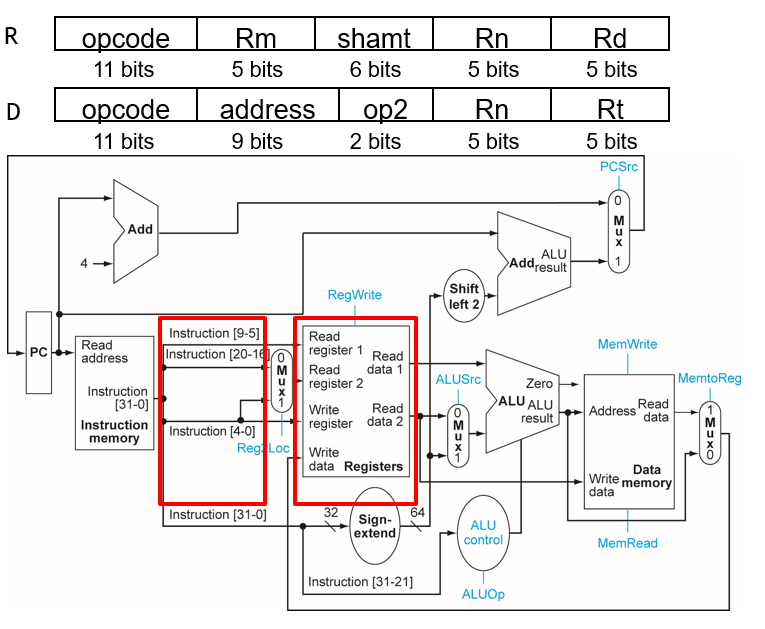
\includegraphics[width=4.75in]{../images/register_file_cutout.png}
	\end{center}
\end{figure} 


\clearpage
\section{Your Assignment}

You are to:
\begin{enumerate}
\item Create an instr\_parse module as described above.
\item Create and Expected Results Table for instr\_parse\_test.
\item Use the instr\_parse test module and verify that the instruction is being parsed properly by comparing to the Expected Results Table.
\item Create a regfile module.
\item Create a regfile\_test module.
\item Create an Expected Results Table for regfile\_test.
\item Verify that the values are being stored and retrieved from the regfile properly by comparing the results with the Expected Results Table.
\item Write a lab report according to the LabN format.
\end{enumerate} 
\chapter{Control Unit and Sign Extender}

\section{Control Unit}
Next, we will create the main control unit.  You will create a new module called control (in control.v) in 2\_decode.  The control module should use a portion of the instruction to determine the values of all control signals to be used in our processor.  These signals include:
\begin{enumerate}
\item reg2\_loc
\item uncondbranch
\item branch
\item mem\_read
\item mem\_to\_reg
\item alu\_op
\item mem\_write
\item alu\_src
\item reg\_write
\end{enumerate}

The supported instructions should include:
\begin{enumerate}
	\item ADD
	\item SUB
	\item AND
	\item ORR
	\item LDUR
	\item STUR
	\item CBZ
	\item B
\end{enumerate}

You will need to evaluate the incoming opcode and set the value of the control lines according to Figure~\ref{fig:control_value_table}.  Note that a value of X in a table entry indicates that it does not matter whether the value is 0 or 1.  You do not want to use X in these cases, as this indicates 'undefined' to Verilog.  Instead, please use 0 in place of X.

\begin{figure}
	\caption{Control Value Table}\label{fig:control_value_table}
	\begin{center}
		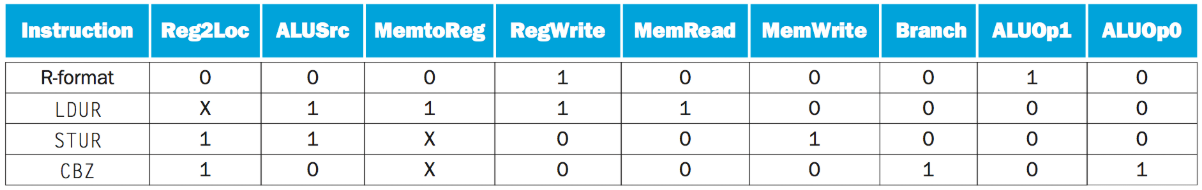
\includegraphics[width=4.75in]{../images/control_value_table.png}
	\end{center}
\end{figure} 

\section{Control Unit Test}
The Control Unit is crucial to operation of your datapath, so it needs to be tested thoroughly.  Every supported instruction (listed above) should be tested with the Control Unit Test.  To facilitate testing, I have provided an Expected Results Table with 10 instructions listed across the top (ARM-Lab/testfiles/ExpectedResultsTable.xlsx).  These are the instructions that you should use to test your Control Unit and your full Decode stage (once we finish it).  The rows of the table are signals that will be inputs and outputs of the control module.  

Before writing your unit test, you should fill in every cell in this table with the expected results.  This includes producing the machine code for each instruction.  Then, use the necessary bits of these machine code instructions as inputs to your Control Unit Test and verify the outputs.  You should display the outputs on your simulation results in the same order that they are shown on the Expected Results Table.  Then, you can go right down the table and easily verify that your results are correct.  

Save the Expected Results Table on GitHub, because we will be adding to it in future labs.  Note that for this lab, you do not need to have time values at the top of your expected results tables.  The instructions give us sufficient granularity.

Note that, at this point, the values that are loaded in the registers do not matter, as we are just testing the Control Unit.  Once we get to the full iDecode stage, we will need to address the register values.

The Verilog implementation between 'if/else' statements and 'case' statements differ.  'If/else' statements will create a series of nested muxes with two inputs each, whereas a case statement will produce one large mux with many inputs.  To maximize speed, we should use case statements. Note that all Verilog case statements must have a default case. But one of the challenges of this lab is dealing with opcodes of different sizes.  Thankfully, Verilog has 'casex', which will only evaluate binary digits that are not labeled X.  So for a CBZ instruction, you can fill in the last 3 digits with XXX and use 'casex'.  The 'casex' syntax will also be very helpful in the Sign Extender.  Also, please create macros in definitions.vh for the opcodes of each instruction and for the ALU Op values of each instruction type.  The values in the macros can include X's when necessary.

\section{Sign Extender}
The final major component of the Decode stage is the Sign Extender.  The Sign Extender should use information in the instruction to create a 64-bit output value to use as an address or branch offset.  You need to extract the constant value from the instruction (this will be different for each instruction type), place that extracted value in the least significant bits of the sign\_extended\_output, then sign extend that value.  For positive values, the sign extender should fill extended bits with 0s.  For negative values, the sign extender should fill the extended bits with 1s.  The sign extender should support extending address values from the following instructions:
\begin{enumerate}
	\item LDUR
	\item STUR
	\item CBZ
	\item B
\end{enumerate}

\section{Sign Extender Test}
The Sign Extender Test should utilize the instructions from the Control Unit test.  Verify that your Sign Extended Output on the Simulation Results matches the value on your Expected Results table.  Instructions that don't use a Sign Extended Output (like R-Type) should fall into the default case.  Fill in the Expected Results Table with the default value.   Note that for this lab, you do not need to have time values at the top of your expected results tables.  The instructions give us sufficient granularity.

\clearpage
\section{Your Assignment}

You are to:
\begin{enumerate}
\item Fill in the entire Expected Results Table, starting with the version that I provide in the testfiles section in GitHub.
\item Create a Control Unit module.
\item Create a Control Unit Test and verify that the simulation results match your Expected Results Table.
\item Create a Sign Extender module.
\item Create a Sign Extender Test Module and verify that the simulation results match your Expected Results Table.
\item  Write a lab report according to the LabN format.
\end{enumerate} 
\chapter{Finishing Decode}

\section{iDecode Module}
At this point, you have created all of the modules necessary to assemble the iDecode module.  Now you need to create a new module called iDecode.  The inputs and outputs can be determined by evaluating Figure~\ref{fig:decode_stage}.  Any signal that crosses the boundaries of the red box is an input or output.  Signals that do not cross the boundaries of the red box are signals that are internal to the iDecode module and should be declared internally in iDecode.  Please make sure to label signals consistently with lower case letters with words separated by underscores.  For example, read\_data1, write\_data, alu\_src.

\begin{figure}
	\caption{Expected Results}\label{fig:decode_stage}
	\begin{center}
		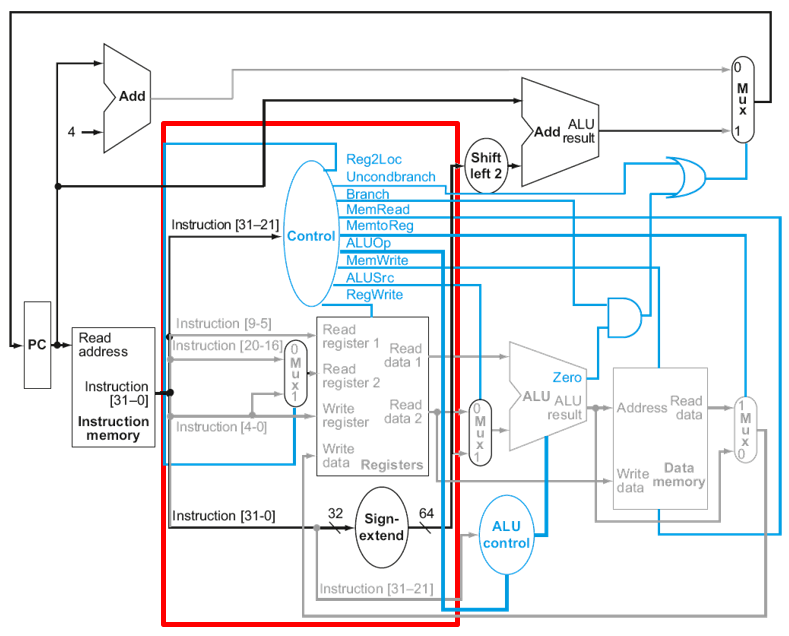
\includegraphics[width=4.75in]{../images/decode_stage.png}
	\end{center}
\end{figure} 


\section{iDecode Unit Test}
To verify that your iDecode module works correctly, you must first update your Expected Results Table. You should first add a row for every input and output of your iDecode module, then fill in all cells with expected values.  If a particular data item is not relevant for a particular instruction (for instance, sign\_extended\_output on an R-type instruction), then just put an X in that cell.  To ensure that we are testing each case, please update regData.data to reflect the following values:

\begin{enumerate}
	\item X19 = 10
	\item X20 = 30
	\item X21 = 0
	\item X22 = 16
\end{enumerate}

Now create a unit test for iDecode by providing the inputs for iDecode and verifying the outputs of iDecode.  For the instruction input, use the instructions from your Expected Results Table.  For arithmetic instructions, use the test bench to provide the correct value to the write\_data input, since we do not yet have an ALU to do the calculations.  Also, please use your test bench to provide a value of 20 to X9 in the first command (LDUR).

With your Expected Results Table in hand, you should be able to run the iDecode unit test and analyze your simulation outputs by going vertically down the simulation output, comparing the table to your simulation output.  While certain values will be offset in time, a single instruction should fall within a single clock cycle.  

\section{Integrating iFetch and iDecode}
Now that you have iDecode created and tested, you can test it with your iFetch module.  To do this, you need to create a file called datapath.v.  This will be your top-level file for your integrated datapath, and it is also the test bench.  In this file, you should have an instance of iFetch and iDecode.  You should connect these two modules with wires by analyzing the full datapath diagram.  Since we do not have a full datapath yet, we need to manipulate some values in datapath.v.  Once the datapath is complete, there will be no need to manipulate values because everything will be connected.  Similarly to your iFetch test, you will want to create a reg for reset, pc\_src, and branch\_target.  Since we do not have all aspects of branching implemented, please keep pc\_src set to 0 for the duration of the test.  You will also need to provide values for write\_data since we do not yet have the stages that produce the value for write\_data.  

Please update your instrData.data file to only contain the 10 instructions in your Expected Results Table.  The goal of datapath.v is to verify that the PC increments, each of these instructions is fetched at the appropriate time, and that the instruction is decoded properly.  You can verify the execution by comparing your results with your expected results table.     

\section{Your Assignment}

You are to:
\begin{enumerate}
\item Integrate all individual modules into the iDecode module.
\item Update your Expected Results Table to include all iDecode inputs and outputs.
\item Test the iDecode module with the instructions from the Expected Results Table.
\item Verify that your simulation results match your expected results.
\item Create datapath.v and integrate the iFetch and iDecode stages.
\item Verify that the results match the Expected Results Table.
\item Write a lab report according to the LabN format.
\end{enumerate} 
%\chapter{ALU and ALU Control}
The goal of this lab is to build the ALU and ALU Control modules. These modules can be seen in the context of the datapath by viewing the datapath diagram from the previous lab, Figure~\ref{fig:decode_stage}.  The ALU performs the arithmetic and logical operations, and the ALU Control module determines which operation should be performed by the ALU.  During this lab, we will not put these modules together.  Instead, they will be tested independently of each other.
\section{ALU}
The ALU has three inputs:
\begin{enumerate}
	\item a\_in - the first input operand
	\item b\_in - the second input operand
	\item alu\_control - control signal used to tell the ALU what operation to perform
\end{enumerate}
The ALU has two outputs:
\begin{enumerate}
	\item alu\_result - the result of the arithmetic/logic operation
	\item zero - a flag indicating whether alu\_result is zero
\end{enumerate}  
Figure~\ref{fig:alu_control_table} identifies the operation that corresponds to the alu\_ctrl value.  You should use a case statement to evaluate the alu\_control bits to determine which ALU operation to perform.  For each operation, you do not have to do anything fancy.  You just need to use the math capability that verilog provides to make the calculation.  To make the code readable, you must give the the ALU control bits names in the definitions.vh file, and you should use these in your cases.  Also don't forget to make a default case, which is needed to actually wire this up.  Pick something fast for the default, thus usually a logic statement.

One last thing to note is the generation of the zero flag.  The zero flag is determine by simply evaluating the alu\_result.  There are several ways to handle this, but the easiest way to handle it is below: 
\begin{enumerate}
\item In Verilog (like C), the statement $(y==0)$ is an operation with a boolean output.  You can thus say $x=(y==0);$ to assign $x$ to be the boolean value that $(y==0)$ produced.  The statement $x=(y==0);$ is realizable as a digital comparator with $y$ and $0$ as inputs and $x$ as the single bit output.
\end{enumerate}

\begin{figure}
	\caption{ALU Control Values}\label{fig:alu_control_table}
	\begin{center}
		\includegraphics[width=2.75in]{../images/alu_control_table.png}
	\end{center}
\end{figure} 

\section{ALU Control}
The ALU Control module has two inputs:
\begin{enumerate}
	\item alu\_op - 2 bit signal giving incomplete information about what ALU operation should be performed
	\item opcode - the opcode of the instruction
\end{enumerate}
The ALU Control module has one output:
\begin{enumerate}
	\item alu\_control - control signal used to tell the ALU what operation to perform
\end{enumerate}
Please define the ALU Op constants and ALU Control constants in definitions.vh file to improve readability.  Figure~\ref{fig:alu_control_table} identifies the operation that corresponds to the alu\_ctrl value.  This module can be implemented multiple ways, but we want to use the most efficient way possible.  The most efficient method is to use a casex statement to evaluate the alu\_op signal, utilizing the information in Figure~\ref{fig:alu_op_opcode_table}.  alu\_op will provide all information necessary for D-Type and CB-Type instructions.  For R-Type instructions, you should use the bits of the opcode to set the alu\_ctrl value.  When evaluating Figure~\ref{fig:alu_op_opcode_table} for R-Type instructions, certain bits of the instruction correspond to alu\_ctrl bits.  The magic decoder ring is listed below.  Please note that the numbering system for the instruction bits includes the entire instruction, whereas you will just have the opcode to work with.  Therefore, you will need to adjust the numbering to account for your 11-bit opcode.
\begin{enumerate}
	\item ALU Ctrl [3] = 0
	\item ALU Ctrl [2] = I[30]
	\item ALU Ctrl [1] = I[24]
	\item ALU Ctrl [0] = I[29]
\end{enumerate} 

\begin{figure}
	\caption{ALU Op Table}\label{fig:alu_op_opcode_table}
	\begin{center}
		\includegraphics[width=4.75in]{../images/alu_op_opcode_table.png}
	\end{center}
\end{figure} 

\section{Your Assignment}

You are to:
\begin{enumerate}
\item Create the ALU module.
\item Create an ALU testbench to test all ALU operations, including testing the zero bit.
\item Create an ALU Control module.
\item Create an ALU Control testbench to test all of the opcode/ALUOp pairs that will be used in our instruction subset.
\item You do not need to create Expected Results tables for these tests, as they are very short and simple.
\item Create a lab report in the LabN format.
\end{enumerate} 
%\chapter{Execute Stage}

\section{Execute}

In the last lab, you created the ALU and ALU Control modules.  Now we will finish the iExecute stage.  The iExecute stage is represented by the red box in Figure ~\ref{fig:execute_stage}.  To finish the iExecute stage, you will need to add the following:
 
\begin{enumerate}
	\item Mux to select the source of the second input into the ALU.  You can reuse your mux that you created in the iFetch stage.
	\item Shifter to left shift the sign extended branch address offset.  You will need to create a new module for this.
	\item Adder to add the branch address offset to the current PC.  You can reuse your adder that you created in the iFetch stage.
\end{enumerate} 

\begin{figure}
	\caption{Execute Stage}\label{fig:execute_stage}
	\begin{center}
		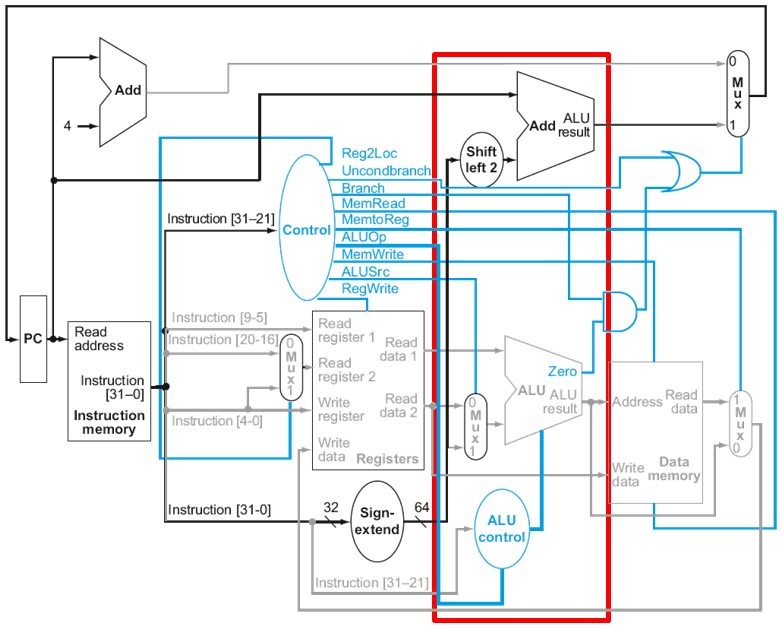
\includegraphics[width=4.75in]{../images/execute_stage.png}
	\end{center}
\end{figure} 

These five modules should be included in a new module called iExecute.  iExecute should consist of everything shown in the red box on Figure ~\ref{fig:execute_stage}. 

\section{Your Assignment}
I have provided a test bench, iExecute\_test.v.  Feel free to modify and improve it as you see fit.

\Verilog{iExecute Test Bench}{code:iExecute_test}{../code/3_execute/iExecute_test.v}

You are to:
\begin{enumerate}
\item Complete the iExecute module 
\item Use the iExecute\_test to create an Expected Results Table.  In the table, just have a column for each clock cycle, since each instruction is executed in one clock cycle.
\item Verify that your simulation results match your expected results.
\item Create a lab report in the LabN format.
\end{enumerate} 
%\chapter{Integrating Fetch and Decode}

\section{Integration}
We now have working Fetch, Decode, and Execute modules.  Now it is time to put them together to produce a system that can:
\begin{enumerate}
	\item Update the program counter
	\item Read the appropriate instruction from the instruction datafile
	\item Read the correct registers
	\item Update all control lines
	\item Sign extend address data
	\item Calculate Branch Target Addresses
	\item Provide a zero bit for conditional branch instructions
	\item Produce ALU results for R-Type and D-Type instructions
\end{enumerate}

Once we can do all of this, we will be ready for the iMemory stage.  We currently have the fetch and decode module integrated into datapath.v.  We also have a working execute module.  Today we need to integrate the Execute module into datapath.v.  Please reuse the instructions from your Expected Results Table that you used when you integrated fetch and decode.  Please make sure that datapath.v is the "top module" in your project.  Once integrated, you should be able to produce a simulation that includes 3 new outputs:
\begin{enumerate}
	\item Branch Target
	\item ALU Result
	\item Zero
\end{enumerate}   

These three new outputs are marked on Figure Figure ~\ref{fig:integrated_execute}.  To verify these outputs, you should update the Expected Results Table to include these three outputs.  Then you should verify this table against your simulation results.

\begin{figure}
	\caption{Execute Stage}\label{fig:integrated_execute}
	\begin{center}
		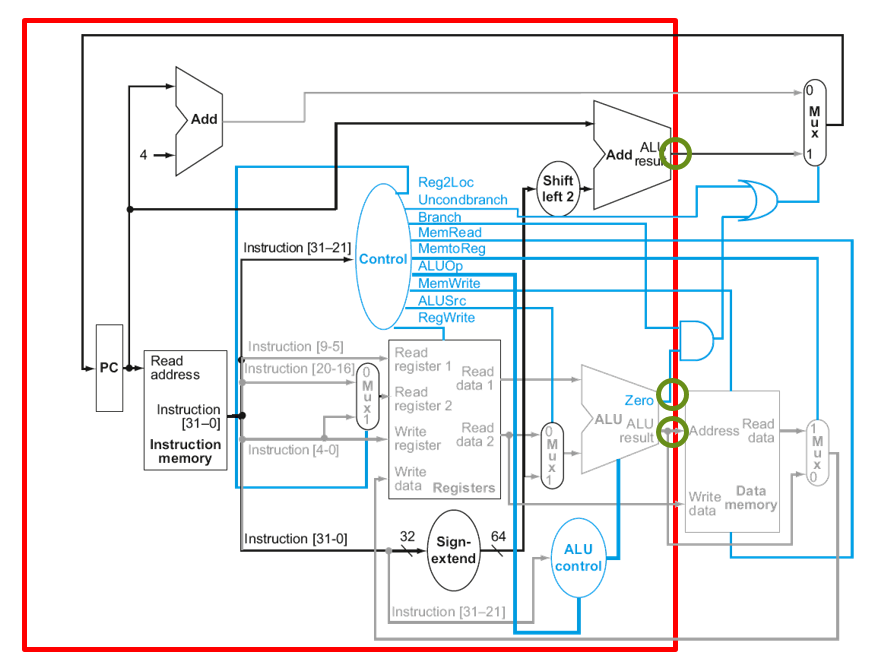
\includegraphics[width=4.75in]{../images/integrated_execute.png}
	\end{center}
\end{figure} 

\section{Your Assignment}

You are to:
\begin{enumerate}
\item Integrate your iExecute module into your datapath.v that includes iFetch and iExecute.
\item Update your Expected Results Table to include the new outputs.
\item Verify that your simulation results match your expected results.
\item Create a lab report in the LabN format that focuses on the integration of the iExecute stage.  The only inputs that you need to list are the inputs that you set in the initial section of datapath.v.  The only outputs are the signals that are leaving the red box in Figure ~\ref{fig:integrated_execute}. 
\end{enumerate}
%\chapter{Memory}

\begin{center}
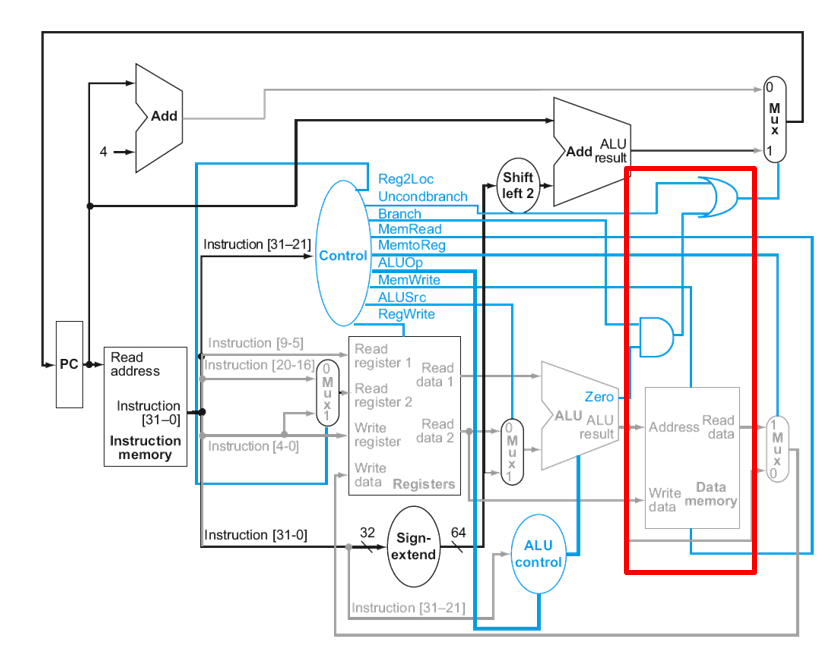
\includegraphics[width=5.5in]{../images/data_memory.png}
\end{center}

\section{Memory Stage}
Today we will create the iMemory stage of our processor.  This stage contains the data memory for the system that we use for load and store commands.  It also contains the logic gates used to produce the pc\_src signal that is used in the iFetch stage.  Note that although the diagram shows the pc\_src mux on the right side of the diagram, the mux is actually already implemented in the iFetch stage and belongs in the iFetch stage.

\section{Branch Resolution}

We now have all the information necessary to decide if the computer should branch or not.  We have the signal `branch' to tell us if it is a branch command, and we have `zero' to tell us if the condition was met.  Both branch and zero must be true so we will combine them with an `and' gate.

We also need an 'or' gate to 'or' together the output of the branch 'and' gate (above) and the uncondBranch control signal.  These gates can be included in your iMemory module as one line commands.  They do not need to be explicity tested, as they will be thoroughly tested when we integrate the system.  

\section{Data Memory}

This will be similar to the register file memory, with two primary changes:
\begin{enumerate}
\item reading is now conditional on the MemRead control wire being high.  If the MemRead flag is not high, then the read\_data output should be set to Z (high impedance).
\item writing is now permissible if the MemWrite control wire is high.
\end{enumerate}
Create a data\_mem.v file, copy the contents of your register file memory and modify it to meet the needs of the data memory module.

\section{Your Assignment}

You are to:
\begin{enumerate}
\item Create a new module called iMemory.
\item Instantiate the AND and OR gates directly in the iMemory stage.
\item Create a new module called data\_mem to handle data memory access.  Also create or modify a ramData.data file that contains initial values to be read into memory.
\item Integrate data\_mem into the iMemory stage.  
\item Write a testbench to verify that the iMemory stage works properly. Use a combination of ramData.data and testbench to test various scenarios.  Make sure to use STUR instructions to set values in memory locations, then read those values back using the LDUR function. 
\item Create a lab report in the LabN format.
\end{enumerate} 
%\chapter{Write Back}


\begin{figure}
\caption{Write Back}\label{fig:wb}
\begin{center}
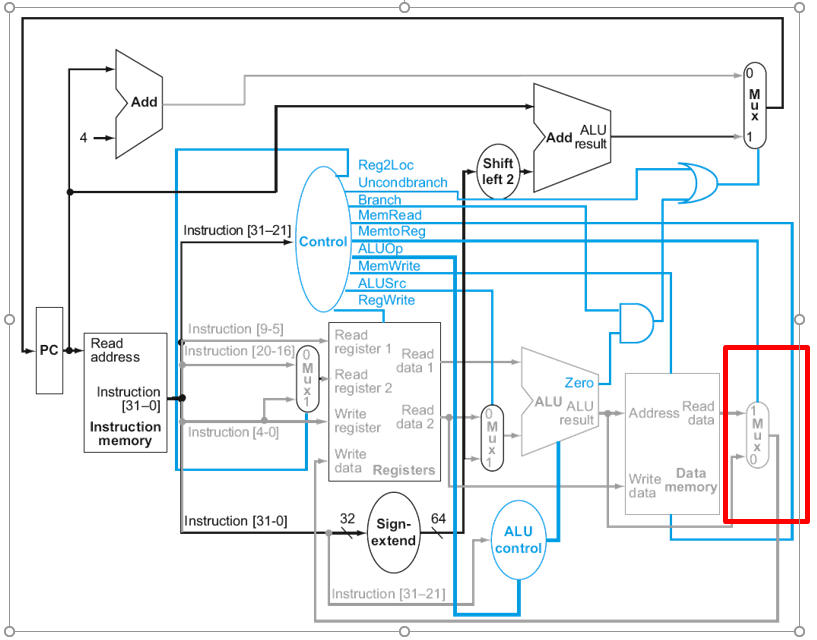
\includegraphics[width=\textwidth]{../images/writeback_stage.png}
\end{center}
\end{figure}

\WrapBarrier

\section{Mux}
This stage consists on only one item, a mux to select between the output of memory and the output of the ALU.  The control is the MemtoReg control line, see Fig~\ref{fig:wb}.  Since the mux has already been tested it does not need a testbench.  The stage thus has only 3 inputs (2 data and 1 control) and one output, the result.

\section{Datapath}
You are ready to assemble the full non-pipelined datapath shown in Fig~\ref{fig:datapath}.  To do this, you will need to combine all 5 stages into datapath.v.  Stages include:
\begin{enumerate}
\item iFetch
\item iDecode
\item iExecute
\item iMemory
\item iWriteBack
\end{enumerate} 

Verify by running your set of instructions in instrData.data and testing the output.  Pay particular attention to make sure that the Rd register is updated appropriately by R-Type and D-Type instructions.  You should no longer set write\_data in datapath.v.  Rather, you should connect write\_data from the WriteBack stage to the Decode stage.  For right now, keep pc\_src hard-coded to 0 in datapath.v.  Even though we could connect it now, our test instructions are not meant to run like a program and would yield strange results.  Each instruction should execute as expected according to your Expected Results Table.  Datapath.v should be your top-level Verilog file (no additional test drivers are necessary).

\begin{figure}
\caption{Full Non-Pipelined Datapath}\label{fig:datapath}
\begin{center}
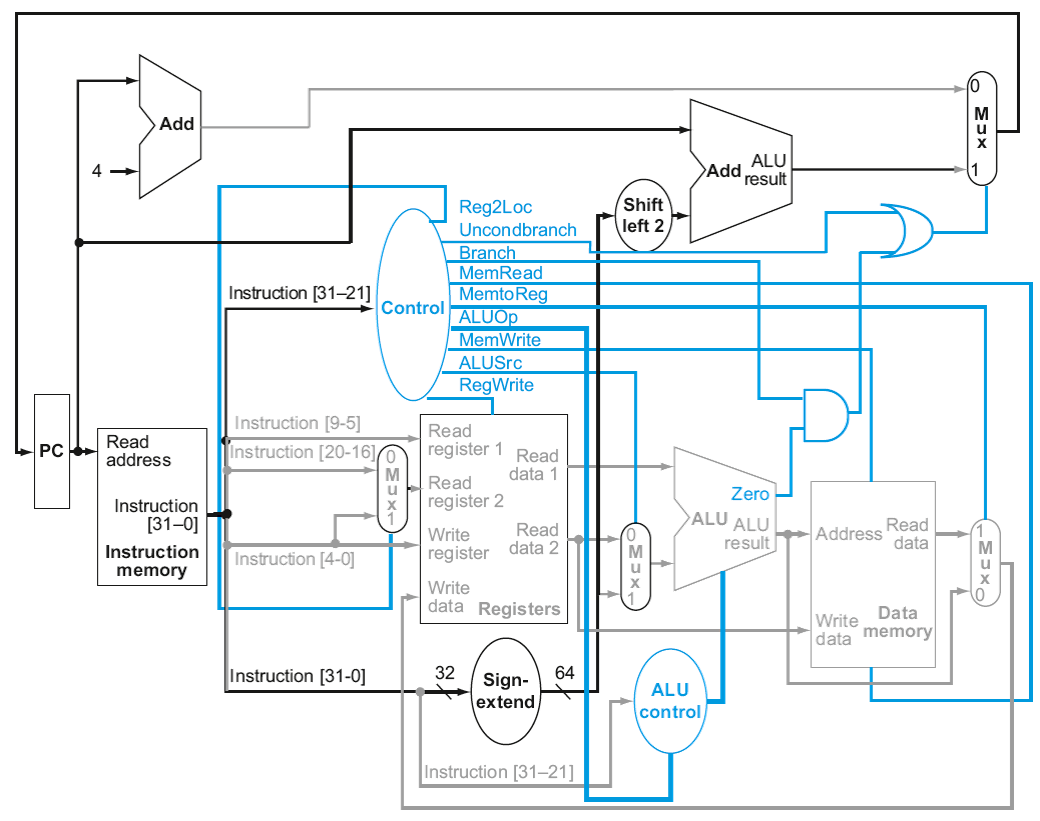
\includegraphics[width=\textwidth]{../images/non_pipelined_datapath.png}
\end{center}
\end{figure}

\section{Your Assignment Part 1}

You are to:
\begin{enumerate}
\item Create the Writeback stage consisting of one Mux.
\item Integrate all five stages into the file datapath.v.
\item Update your Expected Results Table to include the iWriteBack stage.
\item Run simulations to verify that your results match your Expected Results table.   
\item Do not write up a lab report yet. There will be one final test to add before we submit it.
\end{enumerate} 

\section{Division}
To further verify your datapath operation, you should create a new set of datafiles to implement the division code shown below.  You should first write assembly code, then translate it into binary.  One restriction is that the only non-zero value in your regData.data should be X22, which can be used as the base address for the array A.  Otherwise, all other data must be loaded from memory via the ramData.data and LDUR commands.  Please pay attention to the comments in division.c.

\Verilog{C code for doing simple division.}{code:division}{../code/division.c}

\begin{figure}
	\caption{Full Non-Pipelined Datapath}\label{fig:datapath}
	\begin{center}
		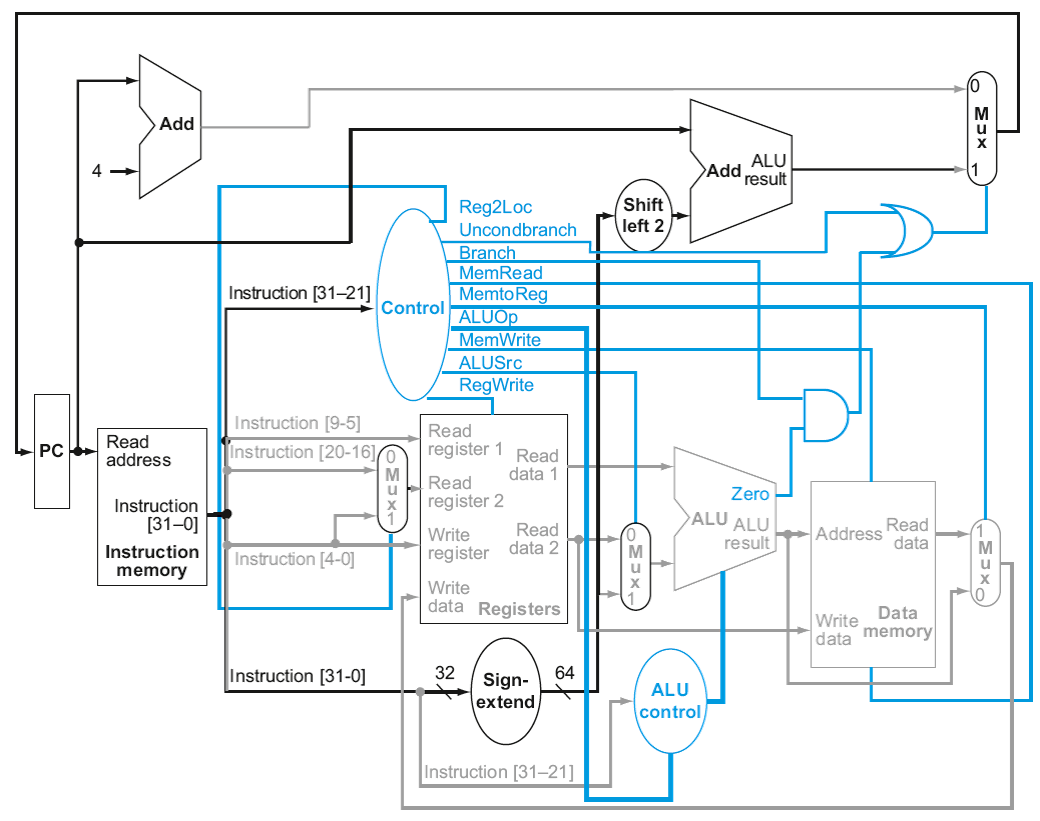
\includegraphics[width=\textwidth]{../images/non_pipelined_datapath.png}
	\end{center}
\end{figure}

\section{Your Assignment Part 2}

You are to:
\begin{enumerate}
	\item Implement the assembly and binary code for the Division C Code shown above.
	\item Verify that the divison works correctly.
	\item Write up a lab report according to the LabN format.
\end{enumerate} 
%\chapter{Pipeline Fetch and Decode}


\section{Pipeline Fetch and Decode}
Now that we have a working single-cycle datapath, we are going to break it apart and start pipelining it.  Make sure to keep a copy of your working single cycle datapath for reference.  To begin the pipelining process, we will first pipeline the iFetch and iDecode stages.

The advantage of pipelining includes the ability to reduce the clock cycle time by doing only one stage at a time.  We have been using a 10ns clock cycle.  Now that we are pipelining, let's start conservative and go down to a 4ns clock cycle.  Please keep it at 4ns for now to maintain consistency across the class.  

This will affect your timing and will require you to update the clocks in your datapath.  The basic clk for each stage should be clk (no delays).  You will still need delayed clocks for items that are delayed within a stage such as read\_clk and write\_clk.  The first goal for your pipeline is to get a series of instructions to execute in pipeline form, where a new instruction is fetched while the previous instruction is being decoded.  You should verify this by examining the Read\_Register values, Read\_Data values, control signal values, etc.  To test this, use your set of instructions that corresponds to your Expected Results table.  For right now, just focus on the Fetch and Decode stages.

\section{Pipeline Buffering and Forwarding}
The next step in developing your pipeline is to add the stage buffers that we have seen in the textbook.  The idea here is that every input to a stage must be buffered so that you do not operate on values that are currently being changed.  The code for this is not complex, but the planning and thought process can be complex because some signals need to be passed through to future stages.  Remember, your signals should only go from one stage to the next stage.  For example, you should not have signals that go from Decode to Memory.  The signal must go from Decode to Execute, then Execute to Memory.  If you skip a stage, the data will be incorrect due to timing issues.  To aid your efforts, I require that you complete the PipelineAnalysisTemplate.xlsx.  This allows you to figure out what signals need to be passed between stages and develops a naming convention that will help you when you start implementing. 

In the spreadsheet, you should start with my template, which has many (not all) of the signals that are in your datapath.  Look at your current connections in datapath.v.  Wherever you see an output from a module, put that in the spreadsheet as a source.  Wherever you see an input to a module, put that in the spreadsheet as a destination.  In many cases, you will see that there is space in the spreadsheet between the source and destination.  This means that the signal must be buffered and forwarded from one stage to the next.  Fill in the space between the source and destination with signals to be forwarded.  Please use the naming convention that I show on the spreadsheet....this might be the most crucial part...even if you don't understand why, just trust me on this one.  The signal names should match your current signal names, but they should have a suffix added to them that indicates which stage outputted the data.  For instance, when mem\_to\_reg was buffered in iExecute and forwarded to iMemory, the signal should be name mem\_to\_reg\_ie because iExecute outputs the data. 


\section{Your Assignment}

You are to:
\begin{enumerate}
\item Save a copy of your non-pipelined datapath.v.
\item Comment out Execute, Memory, and WriteBack stages from datapath.v.
\item Pipeline iFetch and iDecode stages as described above.   
\item Test with your set of instructions from your Expected Results table.
\item Verify that stages are processing the correct instructions at the correct times.
\item Complete PipelineAnalysisTemplate.xlsx
\item Create a lab report with LabN format.
\end{enumerate} 
%\chapter{Pipelining without Branching or Forwarding}


\section{Overview}
Now that we have pipelined the fetch and decode stages, we can add the register buffers between each stage and get a simple pipeline working.  This pipeline will not include any data forwarding or branch prediction.  We will handle data hazards by using assembly code with appropriately placed nop commands.  For now, we will avoid control hazards by keeping pc\_src set to 0, which will keep the system from branching (even when you run a branch instruction).  

Only after you have completed the spreadsheet, then you can move on to writing Verilog code.  You will want to update datapath.v to use the names from the spreadsheet.  This will include adding a lot of new signals.  Then you will want to update your modules to account for these new signals.  Use your spreadsheet to make the following updates:
\begin{enumerate}
	\item Add input ports to stage modules as needed.  This will be particularly relevant for signals that are passed through.  You should not use the \_id, \_ie, etc naming convention within the module.  You should either use no suffix or the suffix \_in or \_out.
	\item Update all modules to buffer all inputs into the module.  This will keep inputs from changing while they are being used.  On the positive edge of the clock, you should use procedural assignments to copy all inputs into another register (reg).  This register can either be an output reg (when appropriate) or a local reg (if the signal does not need to be output).  Then do all of the module's processing on the buffered regs.  Try to change as few names as possible within the modules.  Use names that keep you from having to update your signal names to the lower level modules.  In modules that do not currently have a clock, you will need to add the clock.
	\item Use the information in the spreadsheet to add output ports to stage modules as needed. 
\end{enumerate}
Again, try to change as few names as possible within the modules.  You want to use the stage-specific names (\_ie, etc) in datapath.v rather than in the modules, to the extent possible.

Use the instructions from your Expected Results Table to test your pipeline.  Insert NOP instructions where appropriate in your instrData.data.  To insert a NOP instruction, add a 32-bit line with all zeros.

\section{Your Assignment}

You are to:
\begin{enumerate}
\item Implement the spreadsheet in your datapath.v
\item Update your modules to buffer the appropriate values into registers
\item Use your expected results table instructions to test the pipeline and correct any issues
\item Once your pipeline is working, go back and try to reduce the cycle time as much as possible (without having to re-architect your solution).
\item Submit a lab report using the LabN format.
\end{enumerate} 
%\chapter{Pipelining with Branching}


\section{Overview}
Once your pipeline is working with the simple set of commands that I provided, it is time to add branching.  

We will put the following restrictions on our efforts to branch:
\begin{enumerate}
	\item Use Branch Not Taken method of prediction
	\item You should move the branch decision hardware to the Decode stage as mentioned in the lecture. 
	\item When a branch is taken, you must zero the control lines and set PCWrite and IF/IDWrite to 0.  You will need to add PCWrite and IF/IDWrite.  Branch hazards must be detected by a new module, the Hazard Detection Unit.
	\item Instructions used for this should be the division problem instructions.  You need to insert nops (all zeros) in the instruction file where necessary.  The only reason to add nops in the instruction file is a data hazard
\end{enumerate}  

\section{Your Assignment}

You are to:
\begin{enumerate}
\item Implement Branch Not Taken Prediction
\item Create an instruction file as described above, based on the division problem instruction file
\item Update your modules to detect and respond to branch hazards
\item Use the instruction to test the pipeline and correct any issues
\item Submit picture(s) of your simulation results.  Also submit a zip file of your repository.
\end{enumerate} 

\end{document} 